\documentclass{NEXT-SCNUThesis}

% == 导入额外宏包 ==
% == 一般不用，有报错再补 ==

% =================

\title{Next SCNU Thesis} % 论文题目
\supervisor{xxx} % 指导老师，对于中方版本，中方指导老师在前，英方指导老师在后
\author{郑誉} % 学生姓名
\studentid{20210000000} % 学号
% \institute{xxx} % 学院（未使用）
\major{xxx} % 专业班级
\date{2026年4月} % 论文完成时间

\keywordsen{xxx; xxx; xxx} % 英文关键词
\keywordszh{xxx，xxx，xxx} % 中文关键词（使用全角逗号）

% #########  重要注意事项  ##########
% #################################
% 1. 特别注意图表中的\caption位置,figure的caption要在下方,table的caption要在上方
% 2. 留意Github更新,https://github.com/FaterYU/NEXT-SCNUThesis
% 3. 提交前务必给导师检查
% #################################

% 定义表格标题位置，中方论文在上方
\newif\ifTableCaptionTop
\TableCaptionToptrue

\begin{document}
    \maketitle

    \begin{abstracten}
        The abstract in English goes here. Abstract in English and that in Chinese should agree.
    \end{abstracten}

    \begin{abstractzh}
        这里写中文摘要，中文和英文摘要的内容应该基本对应。
    \end{abstractzh}

    % == 目录 ==
    \toc
    % =========

    % == 正文 ==
    % 在 content 目录下以章节为单位创建 tex 文件，在其中编辑章节内容，并使用 \include{content/xxxx.tex} 插入到这里
    \chapter{Introduction\label{chap:introduction}}

\section{Main Body}

The main body of the thesis constitutes the core of the document and generally consists of five parts: the title, the main text, figures, tables, and equations. The content may vary depending on the nature of the research project, but typically includes theoretical analysis, computational methods, experimental setup and measurement techniques, analysis and discussion of processed experimental results, comparisons with theoretical calculations, and comparisons between the methods used in this study and those of previous research.

The introduction primarily elaborates on the significance of the thesis topic, explaining the necessity, academic value, and practical significance of the research. If the project has a specific background, the source of the project should also be explained.

Furthermore, in conjunction with the proposed topic, a literature review is used to describe the current state of domestic and international research related to the topic, identify existing problems, and thereby propose the research approach of this paper—specifically, what methods and theories will be used to address the problems raised, and what conclusions are expected to be reached. Finally, the main structure of the entire paper is outlined.

\subsection{Sections and Subsections}

You may divide the text into sections or subsections as needed.

\section{Figures, Drawings, Tables and Formulas}

\begin{itemize}
    \item Figures: For referenced figures, indicate the source of the reference in the upper right corner of the figure caption (the textual description of the figure’s content).

    \begin{itemize} 
        \item Figure numbers are assigned sequentially by chapter; for example, Figure 3-2 is the second figure in Chapter 3. If a figure consists of several distinct parts, assign sub-figure numbers (e.g., Figure 3-2a) and provide a caption for each sub-figure.
        \item Add \verb|\label{some-label}| to the figure and use \verb|\ref{some-label}| in the text to automatically reference it, for example, Figure~\ref{fig:example-figure}.
    \end{itemize}

    \item Drawings must be neat, clear, and standardized. Mechanical part drawings must comply with mechanical drafting specifications; schematic diagrams should clearly illustrate the depicted content. Photographs should include a scale bar in the lower right corner.
    \item Tables: Tables are numbered sequentially by chapter; for example, Table 5-4 is the fourth table in Chapter 5. Each table should have a title placed above it.
    This is an example of the Table~\ref{tab:example-table} citation.
\end{itemize}

\begin{figure}[htbp]
    \centering
    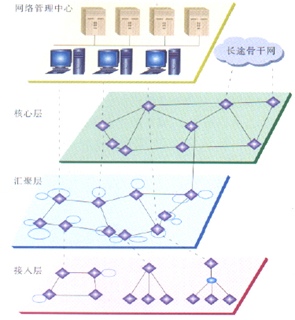
\includegraphics[width=0.5\textwidth]{fig/example.png}
    \caption{Example figure}
    \label{fig:example-figure}
\end{figure}

\begin{table}[htbp]
    \centering
    \caption{Example table}
    \label{tab:example-table}
    \begin{tabular}{|c|c|}
        \hline
        Column 1 & Column 2 \\
        \hline
        Row 1    & Row 2    \\
        Row 3    & Row 4    \\
        \hline
    \end{tabular}
\end{table}


Equations should be placed on a new line within the text. They should be centered, followed by a reference number that corresponds to the chapter sequence and is right-aligned. For papers containing a large number of equations, they may be organized by section, provided that the formatting is consistent throughout the document. For example,
\begin{equation}
    E=mc^{2}
\end{equation}

\section{Citations}

Add citations to reference.bib, then cite one using \verb|\cite{some-cite}|, for example \cite{girshickFastRCNN2015}. You can also use \cite{RussellNorvig2022,vaswaniAttentionAllYou2017} to cite multiple literatures. They will be automatically added to the reference list.
    % =========

    % == 参考文献 ==
    \reference{reference}
    % =========

    % == 附录 ==
    % 在 content 目录下以章节为单位创建 tex 文件，在其中编辑章节内容，并使用 \include{content/xxxx.tex} 插入到这里
    \appendix
    \chapter{User Manual\label{chap:user-manual}}
Please use this template when writing your thesis. However, requirements may vary from year to year, so please refer to the official thesis guidelines and make any necessary adjustments to the template.
    % =========

    % == 致谢 ==
    % 在 content/acknowledgements.tex 中编辑致谢内容，并使用 I would like to express my sincere gratitude to all those who have contributed to the completion of this thesis. First and foremost... 插入到这里
    \acknowledgements
    I would like to express my sincere gratitude to all those who have contributed to the completion of this thesis. First and foremost...
\end{document}